% sphere-cone.tex
\section{Spherically-blunted cone}
%
An aeroshell-type model is shown in Figure\,\ref{sphere-cone-p-fig}.
The surface of the aeroshell is constructed as a \texttt{RevolvedSurface} 
with a sphere blended into a cone.
The construction \texttt{Path} is a \texttt{Polyline} consisting of 
an \texttt{Arc} and a straight \texttt{Line}.
The outer (inflow) surface of the block is constructed by revolving a spline
(approximating Billig's shock shape) about the $x$-axis. 
For specifying the flow domain, only subsections of these surfaces were used
(as \texttt{MappedSurface} objects) as opposite sides of the single block
grid.
The remaining four surfaces were constructed by joining the edges and corners
of these two original surfaces.
During the development of this example, it was useful to view parts of the
constructed paths and surfaces and a later section of the input script shows
how the objects can be rendered to a Virtual Reality Markup Language (VRML)
file.
Although, not as convenient as a direct-manipulation graphical interface, this
rendering facility does enable the debugging of fairly complex constructions.

\begin{figure}[htbp]
\mbox{
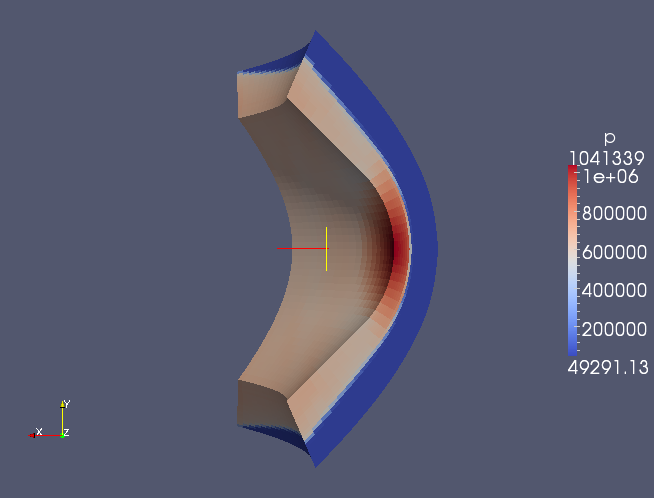
\includegraphics[width=0.5\textwidth]{../3D/sphere-cone/sphere-cone-p-field-from-inside.png}
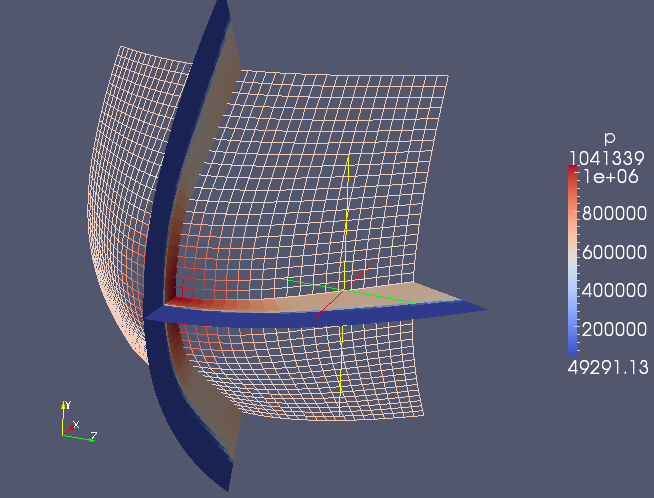
\includegraphics[width=0.5\textwidth]{../3D/sphere-cone/sphere-cone-p-slices-with-mesh.png}
}
\caption{Views of the pressure field around a spherically-blunted cone.
  The left figure is the cell-average data for the entire block rendered as a
  coloured surface.  The view is from behind the aeroshell surface.  Only one
  half of the \texttt{RevolvedSurface} was used in the simulation.
  The right figure shows two cutting planes through the block of data,
  coloured according to pressure, again.
  The surface mesh corresponds to the EAST boundary surface of the block
  and is shown with its mirror image in the (x,y)-plane.}
\label{sphere-cone-p-fig}
\end{figure}

\medskip
For the $20 \times 20 \times 40$ grid and requested final time of 5\,ms 
in this simulation, the run time was a fairly short 9m8.5s on geyser.
(Compare with \texttt{Elmer2}, which used 3m57s on the LG LS70 laptop for the same exercise.)
The grid generation phase takes a relatively long time because of the implied nested function calls
required by the interpolation procedure when using mapped surfaces and paths 
defined on those mapped surfaces.
For finer grids, the grid generation will become quite slow but it is a
once-off cost.

\newpage
\subsection{Input script (.py)}
\index{geometric element!MappedSurface!example of use}
\index{geometric element!RevolvedSurface!example of use}
\topbar
\lstinputlisting[language={}]{../3D/sphere-cone/sphere-cone.py}
\bottombar
